%--------------------------------------------------------------------------------------------------
% ips-msc-thesis-eng-ieee.tex v1.3 (see the end of the file for modification history)
% To be used with ipsthesis.cls v1.3
% 
% A template for creating a MSc thesis in English using the IEEE reference formatting with several 
% accompanying files.  
% By Tea Tušar <tea.tusar@ijs.si>
%
% IMPORTANT NOTE: Biber must be used as the backhand for processing bibliographies, not bibtex!
%
% To compile this template, you need to run the following sequence of commands:
% 1. pdflatex  ips-msc-thesis-eng-ieee
% 2. biber     ips-msc-thesis-eng-ieee
% 3. makeindex ips-msc-thesis-eng-ieee (optional, if you want an index)
% 4. pdflatex  ips-msc-thesis-eng-ieee 
% 5. pdflatex  ips-msc-thesis-eng-ieee
%--------------------------------------------------------------------------------------------------
\documentclass[msc,eng,ieee]{ipsthesis}
%
%--------------------------------------------------------------------------------------------------
%  
% PREAMBULE
%--------------------------------------------------------------------------------------------------
%
% Files with bibliographies 
\addbibresource{references.bib}
%
% Define here all other packages and commands you need for your thesis, for example:
\usepackage{color}
\usepackage{longtable}
%--------------------------------------------------------------------------------------------------
%  
% DOCUMENT
%--------------------------------------------------------------------------------------------------
\begin{document}
%--------------------------------------------------------------------------------------------------
%
% The cover page and spine are created separately using two .doc files provided by IPS.
%--------------------------------------------------------------------------------------------------
%
% FRONT MATTER
%--------------------------------------------------------------------------------------------------
%
\frontmatter
%
\selectlanguage{american}
\pagestyle{fancy}
%
% Title pages
%--------------------------------------------------------------------------------------------------
% 
% INPUT FOR THE TITLE PAGES
%--------------------------------------------------------------------------------------------------
% 
% Author
\author{Klemen Kubelj}         
%
% Title in English (use \protect\\ instead of \\ to create a line break)
\titleEnglish{Physical climate risk: Flood Model Comparison, Hazard and Vulnerability Assessment and Financial Implications}
%
% Title in Slovene (use \protect\\ instead of \\ to create a line break)
\titleSlovene{Naslov v slovenščini}
%
% Supervisor (title and name, affiliation)
\supervisorOne{Prof.\ Mitja Luštrek}{Institut Jožef Stefan, Ljubljana, Slovenia}
%
% Co-supervisor (title and name, affiliation), optional
\supervisorTwo{Prof.\ Boštjan Kaluža}{Arvio d.o.o, Ljubljana, Slovenia}
%
% Co-supervisor (title and name, affiliation), optional
%\supervisorThree{Prof.\ Name Surname3}{Institution3, Place, Country}
%
% Evaluation board chairman (title and name, affiliation)
\evaluationBoardChairman{Prof.\ dr.\ Mitja Luštrek}{Institut Jožef Stefan, Ljubljana, Slovenia}
%
% Evaluation board member #1 (title and name, affiliation)
\evaluationBoardMemberOne{dr.\ Tea Tušar}{Institut Jožef Stefan, Ljubljana, Slovenia}
%
% Evaluation board member #2 (title and name, affiliation)
\evaluationBoardMemberTwo{dr.\ Inna Novalija}{Institut Jožef Stefan, Ljubljana, Slovenia}
% 
% Date
\thesismonth{Month}
\thesisyear{Year}
%
\maketitle 
%
% Dedication (optional)
% %--------------------------------------------------------------------------------------------------
% 
% INPUT FOR THE DEDICATION
%--------------------------------------------------------------------------------------------------
\dedication{To my family and friends}
\makededication
%
% Acknowledgments
\input{text-eng/front-acknowledgments}
% 
% English abstract
%--------------------------------------------------------------------------------------------------
% 
\chapter*{Abstract}
\pdfbookmark[0]{Abstract}{Abstract}
%--------------------------------------------------------------------------------------------------
Flooding is one of the most frequent and damaging natural hazards globally, and its risk is projected to increase due to climate change. Accurate flood risk assessments are essential for spatial planning, climate adaptation, and ESG-aligned financial decision-making. This thesis investigates physical flood risk by comparing global and local hazard models, evaluating standardized vulnerability functions, and quantifying financial implications for real estate assets in Slovenia.

Two flood hazard models are assessed: the global WRI Aqueduct River Flood model and the high-resolution local model Integralna karta globin (IKG). A geospatial validation dataset comprising flood depth and damage records from four flood events in Slovenia (2010--2023) is used to evaluate model accuracy. Flood depths are analyzed using both regression and classification metrics, while vulnerability is assessed through comparison of observed damages against standardized depth--damage functions provided by the European Commission Joint Research Centre (JRC).

A key technical contribution is the development of a data processing pipeline that harmonizes heterogeneous IKG hazard data and integrates it into the modular Physrisk platform using the Zarr data format. This enables scalable, scenario-based risk assessment and model intercomparison.

Findings suggest that while local models offer improved accuracy for continuous flood depth prediction in regression tasks, the global model performs better in categorical classification. Proximity to water bodies was not found to significantly improve prediction accuracy. Depth--damage functions align well with observed damage distributions for residential properties, though segmentation by property type reveals variability in model performance.

The thesis contributes to the validation and integration of physical climate risk models for real estate applications and supports the advancement of ESG-compliant climate risk disclosures.

%
% Slovene abstract, switch to slovene
\selectlanguage{slovene}
\input{text-eng/front-abstract-slo}
\selectlanguage{american}
%
% Contents
\maketoc
%
% List of figures (required if the thesis contains figures)
\makelof
%
% List of tables (required if the thesis contains tables)
\makelot
%
% List of algorithms (required if the thesis contains algorithms)
\makeloa
%
% Abbreviations (optional)
%--------------------------------------------------------------------------------------------------
% 
\chapter{Abbreviations}
%--------------------------------------------------------------------------------------------------
%
% A command that adjusts the of vertical positioning in the abbreviations and symbols chapters
\chapteradjust
% Correct the width of columns (23pt and 377pt) to fit your needs (they should sum up to 400pt).
% Use \cr instead of \\ to break lines.
\begin{longtable}{@{}p{23pt}@{\hspace{2pt} \dots \hspace{5pt}}p{377pt}@{}}
JSI	& Jožef Stefan Institute \cr
IPS & International Postgraduate School \cr
AEP & Average Exceedance Probability \cr
EAD & Expected Annual Damage \cr
ESG & Environmental, Social, and Governance \cr
JRC & Joint Research Centre \cr
RP & Return Period \cr
WRI & World Resources Institute \cr
\end{longtable}
%
% Symbols (optional)
%--------------------------------------------------------------------------------------------------
% 
\chapter{Symbols}
%--------------------------------------------------------------------------------------------------
%
% A command that adjusts the vertical positioning in the abbreviations and symbols chapters
\chapteradjust
% Correct the width of columns (10pt and 390pt) to fit your needs (they should sum up to 400pt).
% Use \cr instead of \\ to break lines.
\begin{longtable}{@{}p{10pt}@{\hspace{2pt} \dots \hspace{5pt}}p{390pt}@{}}
% $j^\star$	& black-body irradiance \cr
% $\sigma$	& Stefan's (or Stefan-Boltzmann) constant \cr
% ---- Flood Risk ----
$h$	& flood depth (m) \cr
$D$	& relative damage (0-1) \cr
$\Omega$ & study area \cr
$E$ & property value (€) \cr
$RP$ & return period (years) \cr
$AEP$ & average exceedance probability (\%) \cr
$EAD$ & expected annual damage (€) \cr
\end{longtable}
%
% Glossary (optional)
\input{text-eng/front-glossary}
%--------------------------------------------------------------------------------------------------
%
% MAIN MATTER
%--------------------------------------------------------------------------------------------------
%
\mainmatter
%
% Introduction
%--------------------------------------------------------------------------------------------------
\chapter{Introduction}
%--------------------------------------------------------------------------------------------------

\section{Background and Motivation}

Flooding is a major natural hazard, responsible for substantial economic losses, social disruption, and loss of life across the globe. With changing climate conditions, flood risks are intensifying in both frequency and magnitude. The Intergovernmental Panel on Climate Change (IPCC) projects a rising likelihood of extreme hydrological events, including both pluvial and fluvial floods, due to higher precipitation variability and rising sea levels.

In Europe, and particularly in Central and Eastern regions such as Slovenia, recent flood events have exposed vulnerabilities in both infrastructure and institutional response systems. The need for robust flood risk models that can inform spatial planning, insurance pricing, and asset management is therefore more pressing than ever. This is especially relevant for stakeholders in the real estate and financial sectors, who must now account for climate-related risks as part of their environmental, social, and governance (ESG) reporting and compliance requirements.

\section{Types of Climate Risk}

In the context of climate-related financial disclosures and scenario analysis, climate risks are commonly categorized into three broad types: \textit{physical}, \textit{transition}, and \textit{liability} risks \cite{moorhouse2024}.

\begin{itemize}
    \item \textbf{Physical risks} arise from the direct consequences of climate variability and long-term climate change. These include acute hazards such as floods, storms, and wildfires, as well as chronic effects such as sea-level rise and shifting temperature regimes. These risks can cause immediate physical damage and long-term degradation of asset value.
    
    \item \textbf{Transition risks} arise from the transition to a low-carbon economy. They include policy changes (e.g., carbon pricing, emissions regulations), technology disruption, evolving market preferences, and reputational risks associated with inaction or misalignment.
    
    \item \textbf{Liability risks} are considered by some \cite{woetzel2020climate} and encapsulate risks arising when those affected by anthoropogenic climate change seek compensation.
\end{itemize}

These categories are increasingly embedded in supervisory and regulatory frameworks, including those developed by the Task Force on Climate-related Financial Disclosures (TCFD) and the Network for Greening the Financial System (NGFS). In the European context, the European Central Bank (ECB) requires significant institutions to assess and disclose their exposure to climate-related and environmental risks, including physical risks, as outlined in its \textit{Guide on climate-related and environmental risks} \cite{ecb2020}. Banks are expected to integrate these risks into their internal governance, risk management, and stress testing frameworks. This thesis focuses exclusively on \textbf{acute physical risks}, with a particular emphasis on riverine flooding and its financial impact on real estate assets.


\section{Climate Risk and the ESG Framework}

As institutional investors and financial regulators increasingly emphasize sustainability, the ESG framework has become a central tool for assessing climate-related risks. The environmental dimension of ESG includes metrics such as energy efficiency, greenhouse gas emissions, biodiversity impact, and—critically—exposure to climate-related hazards.

To operationalize physical risk in quantitative models, it is commonly decomposed into three interacting components:

\begin{itemize}
    \item \textbf{Hazard} – the probability and intensity of a climate-related event (e.g., flood depth for a 100-year return period),
    \item \textbf{Vulnerability} – the expected damage to an asset given the intensity of the hazard,
    \item \textbf{Exposure} – the presence and value of assets located in potentially affected areas.
\end{itemize}

These components form the basis of scenario-based risk models that estimate potential losses under varying climate conditions. However, despite their theoretical appeal, such models often suffer from limited spatial precision, scarce validation against real-world observations, and inconsistent data integration across regions. These issues are particularly acute for flood modeling, where local hydrology and building typologies vary substantially across jurisdictions.

\section{Problem Statement}

While global flood hazard models such as the WRI Aqueduct River Floods provide broad coverage and climate scenario integration, they are often limited in spatial resolution and may not reflect local hydrological conditions. On the other hand, high-resolution local models, such as Slovenia’s \textit{Integralna karta globin} (IKG), offer detailed inundation mapping but are typically fragmented, static (i.e., not climate scenario-aware), and difficult to integrate into broader risk platforms.

Furthermore, flood vulnerability is typically modeled using generalized depth--damage functions derived from empirical or synthetic data. These functions may perform well in aggregate, but their applicability across different building types, geographies, and damage-reporting standards remains uncertain. This creates uncertainty in downstream financial estimates and limits the usefulness of such models for asset-level ESG disclosure.

\section{Research Objectives}

This thesis aims to evaluate the performance of global and local flood risk models with a specific focus on hazard and vulnerability components. The main objectives of the research are:

\begin{enumerate}
    \item To compare the predictive accuracy of flood depth estimates from a global model (WRI Aqueduct) and a high-resolution Slovenian model (IKG) using real flood observations.
    \item To assess how well global depth--damage functions (e.g., from the JRC) reflect reported flood damage across different real estate asset types in Slovenia.
    \item To evaluate whether spatial resolution or proximity to water bodies significantly influence model performance.
    \item To develop and document a data onboarding pipeline that enables integration of heterogeneous local flood maps into the modular \textit{Physrisk} physical risk modeling framework.
\end{enumerate}

\section{Methodological Approach}

The thesis adopts a comparative modeling approach using geospatial and statistical techniques. A validation dataset, compiled from the records of the Slovenian Administration for Civil Protection and Disaster Relief, includes appraised damage and measured flood depths for selected events between 2010 and 2023.

Flood hazard models are evaluated using both regression-based and classification-based metrics to assess depth prediction accuracy. Vulnerability models are tested by comparing observed versus predicted damages using segmented analysis by flood depth and real estate type. All data are processed and harmonized into a common geospatial reference system and stored in Zarr format, enabling scalable access within the \textit{Physrisk} platform.

From a scientific perspective, this work contributes to the empirical validation of global flood hazard and vulnerability models in a local Central European context. From a practical standpoint, it improves the transparency and reusability of flood risk data pipelines, supporting efforts to build ESG-compliant risk disclosure tools.

\section{Structure of the Thesis}

The remainder of the thesis is structured as follows:

\begin{itemize}
    \item \textbf{Chapter 2} presents a review of relevant literature and related work on flood hazard modeling, vulnerability estimation, and ESG-aligned risk frameworks.
    \item \textbf{Chapter 3} describes the study area, datasets, and the methodological framework used for model evaluation and data processing.
    \item \textbf{Chapter 4} details the integration of the local IKG model into the Physrisk framework and presents the architecture of the comparison toolset.
    \item \textbf{Chapter 5} provides experimental results, including quantitative evaluation of model performance, depth--damage function analysis, and financial impact estimates.
    \item \textbf{Chapter 6} discusses the key findings, limitations, and possible future research directions, and concludes the thesis.
\end{itemize}



%
% Second chapter 
%--------------------------------------------------------------------------------------------------
\chapter{Literature Review and Related Work}
\label{chap:literature-review-and-related-work}
%--------------------------------------------------------------------------------------------------

This chapter reviews key research and frameworks related to flood risk modeling, with a focus on hazard modeling, vulnerability assessment, exposure estimation, and regulatory context. The literature spans hydrology, geospatial modeling, and financial risk assessment, with special emphasis on tools applicable to European and Slovenian contexts.

%----------------------------------------------------------------------------------------
\section{Flood Hazard Modeling}
%----------------------------------------------------------------------------------------
Flood hazard modeling estimates the spatial extent and intensity of inundation for specified exceedance probabilities or return periods. It provides the foundational input to flood risk assessment by determining where, how often, and how deep flooding occurs under given scenarios. Two broad model families dominate practice: (i) global models designed for comparability and scenario analysis, and (ii) high-resolution local hydraulic models developed for planning and regulation.

\subsection{Global Flood Models}
Global flood models are designed for consistency and scalability across countries. They typically simulate flood hazard using simplified hydrological and hydraulic methods driven by global datasets such as digital elevation models (e.g., MERIT DEM), river discharge statistics, and climate projections.

One such model is the \textbf{WRI Aqueduct River Flood Model}, developed by the World Resources Institute. It provides flood depth estimates at approximately 1 km resolution for return periods ranging from 2 to 1000 years and supports climate change scenarios such as RCP4.5 and RCP8.5 \cite{wri_aqueduct_floods, ward_aqueduct_2020, kuzma_aqueduct_2023}. The model is designed to support scenario-based stress testing, risk disclosures, and portfolio-level flood exposure estimation. However, its spatial granularity may be insufficient for site-level decision-making or building-level risk evaluation \cite{woetzel2020climate, ipcc2021}.


\subsection{Local Hydraulic Models}

In Slovenia, the national flood mapping programme implements the EU Floods Directive (2007/60/EC) through three products derived from approved hydrological–hydraulic studies (HHS): 
\begin{itemize}
    \item the \emph{integralna karta poplavne nevarnosti} (iKPN; extents for RP10/RP100/RP500)
    \item the \emph{integralna karta razredov poplavne nevarnosti} (iKRPN; hazard classes)
    \item the \emph{integralna karta globin pri Q100} (iKG100; depth classes at RP100)
\end{itemize}

These layers are produced under the responsibility of Ministry of Natural Resources and Spatial Planning, specifically its Water Directorate (\textit{Direkcija Republike Slovenije za vode}), by aggregating and quality-controlling HHS prepared for multiple areas of importance (OPVP).\cite{si_ikg_posodabljanje_integralnih_kart_2015, si_ikg_flood_maps_methodology_2020}. These layers are modeled by certified engineering companies such as DRI d.o.o., iS Projekt, and the Institute for Water of the Republic of Slovenia. National methodology and production process summarized in \cite{si_ikg_posodabljanje_integralnih_kart_2015, si_ikg_flood_maps_methodology_2020,si_ikg_predhodna_ocena_poplavne_ogrozenosti_2019,si_ikg_pravilnik_2007}. Dataset access: \cite{si_ikg_data_2025}.

Flood simulations are based on 1D or 2D hydraulic modeling using high-resolution LiDAR-derived terrain data. The iKG100 depth maps classify inundation into three discrete depth categories: \textbf{Gm} (depth $<0.5$\,m), \textbf{Gs} ($0.5$–$1.5$\,m), \textbf{Gv} ($\ge 1.5$\,m), with a polygon marking the model’s \emph{area of validity} (AOV).\cite{si_ikg_flood_maps_methodology_2020} 

Compared with global models, these local layers provide substantially higher spatial resolution but are not scenario-aware. Although HHs typically produce flood depth estimates for multiple return periods (10, 100, 500 years), the integral depth product (iKG100) is officially published only for RP100 \cite{si_ikg_data_2025}. This represents a technical limitation, which is discussed further in Section~\ref{sec:hazard-data-sources-and-modeling-approach}.

\textit{Use case description from official portal (translated) \cite{si_ikg_data_2025}}:
\begin{quote}
"The core purpose of the IKG data layer is to define spatial restrictions for spatial interventions and land use on areas at risk of flooding. The data also serve for planning flood risk reduction measures, spatial planning, and informing the public about flood risk."
\end{quote}

\subsection{Return Periods and Exceedance Probabilities}

Both global and local models represent flood hazard as a function of return period \( RP \), which reflects the average time between flood events of a given magnitude. The annual exceedance probability (AEP) is defined as:

\[
AEP = \frac{1}{RP}
\]

This mathematical formulation allows different hazard layers to be harmonized and aggregated in subsequent risk calculations \cite{ward_how_2011}.

Recent studies show that the choice and granularity of return periods significantly affect total risk estimates—especially for metrics like Expected Annual Damage (EAD)—emphasizing the importance of high return-period resolution \cite{ward_how_2011}.

\subsection{Climate Scenarios and Hazard Projections}

Flood models increasingly integrate climate scenarios to account for the effects of climate change on future flood hazard. The Representative Concentration Pathways (RCPs) developed by the IPCC serve as standardized radiative forcing trajectories:

\begin{itemize}
    \item \textbf{RCP4.5} assumes stabilization of greenhouse gas emissions, leading to approximately 2.4–3.2\textdegree C warming by 2100.
    \item \textbf{RCP8.5} reflects continued high emissions, potentially leading to >4\textdegree C warming \cite{ipcc2021}.
\end{itemize}

Models like WRI Aqueduct simulate future flood depths under both RCP scenarios, allowing risk analysts to quantify how increasing precipitation, runoff, and sea level may affect hazard exposure in coming decades \cite{bavandi_physical_2022, ipcc2021}.

\subsection{Summary}

Global models offer scalability and scenario coverage but often lack spatial detail. Local models, like Slovenia’s IKG, offer high resolution and contextual accuracy but lack global comparability and scenario flexibility. The choice of model depends on the application—portfolio stress testing may prefer global models, while asset-level analysis or planning benefits from detailed local models \cite{huizinga_global_2017, ipcc2021}.


%----------------------------------------------------------------------------------------
\section{Vulnerability Modeling}
%----------------------------------------------------------------------------------------

Flood vulnerability quantifies the relationship between hazard intensity (typically flood depth) and the resulting damage to physical assets. It is commonly modeled using \textbf{depth--damage functions} (DDFs), which map flood depth to fractional loss of asset value.

\subsection{Types of Depth--Damage Functions}

Depth--damage functions can be derived through various approaches:

\begin{itemize}
    \item \textbf{Empirical DDFs} are constructed from post-disaster damage surveys and insurance claims. While highly context-specific, their availability is often limited due to data confidentiality and geographic constraints.
    
    \item \textbf{Synthetic DDFs} are developed via expert judgment, simulations, or engineering heuristics. These are common in regions without historical damage data and are often used in regulatory frameworks (e.g., HAZUS in the U.S.) \cite{scawthorn_hazus-mh_2006}.
    
    \item \textbf{Standardized global DDFs} offer harmonized vulnerability curves across countries and building types. A notable example is the dataset by the Joint Research Centre (JRC), which includes normalized depth--damage functions and maximum damage values for various assets globally \cite{huizinga_global_2017}.
\end{itemize}

These functions typically start at a threshold depth (e.g., 0.1 m), increase with rising floodwater, and saturate at a maximum loss value (e.g., 70--90\% of replacement value for residential buildings). An example is shown in Figure~\ref{fig:ddf-jrc-europe} in Chapter~3.

\subsection{Use of JRC Vulnerability Curves}

This thesis uses JRC standardized vulnerability functions due to their consistency and availability for European countries. The curves are calibrated to represent fractional damage relative to building replacement value (BRV), making them suitable for property-level assessments across regions \cite{huizinga_global_2017}.

JRC functions are stratified by asset type (residential, commercial, industrial) and were assigned to Slovenian buildings based on available metadata or assumed building usage types in the damage reports.

\subsection{Validation and Regional Applicability}

While standardized functions facilitate large-scale modeling, their accuracy at local levels is not guaranteed. Validation with empirical data is essential.

In this thesis, local flood damage reports from Slovenia (2010--2023) were used to test the applicability of JRC curves \cite{urszr_damage_data}. Reported flood depths and damage amounts were compared to DDF-predicted losses to assess:

\begin{itemize}
    \item The bias and variance of model predictions,
    \item Whether adjustments are needed for specific building types or flood classes,
    \item How well the JRC curves transfer to Central European urban and rural contexts.
\end{itemize}

This approach aligns with recent recommendations on validating vulnerability models using locally observed events and supports adaptation of standardized curves to regional contexts \cite{gentile_scoring_2022}.

\subsection{Uncertainty and Transferability}

One of the key limitations in flood vulnerability modeling is the uncertainty in applying DDFs across different geographies and asset types. Factors such as building materials, maintenance standards, and floor elevation significantly influence damage outcomes but are rarely captured in standardized functions \cite{bressan_asset-level_2024}.

This thesis adopts a conservative approach by applying DDFs to estimate relative (not absolute) damage and focuses primarily on model comparison and validation, rather than financial forecasting. This helps reduce the impact of scale errors and exposure inaccuracies.


%----------------------------------------------------------------------------------------
\section{Exposure Modeling and Financial Risk Metrics}
%----------------------------------------------------------------------------------------

Flood exposure refers to the value and spatial distribution of assets that are potentially affected by flooding. In the context of physical climate risk, it typically denotes buildings, infrastructure, or other economic assets located in flood-prone areas.

\subsection{Asset-Level Exposure Estimation}

Accurate exposure estimation is essential for risk quantification. Methods vary based on data availability and spatial resolution:

\begin{itemize}
    \item \textbf{Cadastral or administrative data} include tax records, property registries, or insurance databases that provide building location and value. These offer the most accurate source of asset-level exposure, but are often limited due to privacy or accessibility constraints.

    \item \textbf{Proxy-based estimates} use geospatial data (e.g., building footprints, land use maps) and assign average values per m\textsuperscript{2} based on construction type or region. These are useful for large-scale or cross-country modeling where granular data is unavailable.

    \item \textbf{Synthetic approaches} simulate building distribution and value using statistical models calibrated on available reference areas. These are common in flood modeling platforms such as HAZUS or GLOFRIS \cite{scawthorn_hazus-mh_2006, ward_assessing_2013}.
\end{itemize}

For this thesis, property values are estimated based on building location and typology, harmonized with the vulnerability curves from JRC \cite{huizinga_global_2017}. Exposure is expressed in relative terms (percentage damage), reducing dependence on exact monetary valuations.

\subsection{Building Replacement Value (BRV) as Exposure Metric}

Many flood loss models define damage relative to the \textbf{Building Replacement Value} (BRV), i.e., the cost to fully rebuild the structure. This standardization allows for comparability across countries and buildings of different ages or materials \cite{huizinga_global_2017, bressan_asset-level_2024}.

BRV-based modeling simplifies vulnerability assignment and integrates well with DDFs. However, it requires assumptions about construction costs and asset characteristics, which introduces uncertainty when applied at national or continental scales.

\subsection{Financial Risk Metrics: Expected Annual Damage (EAD)}

Expected Annual Damage (EAD) is a commonly used financial risk indicator that captures long-term expected flood losses by integrating damage across all modeled return periods.

EAD is computed as the area under the exceedance probability-loss curve (risk curve):

\[
\text{EAD} = \int_0^1 D(h(p)) \cdot E \, dp
\]

This approach is widely recommended in regulatory and scientific literature as it accounts for both frequent low-intensity floods and rare extreme events \cite{ward_how_2011, bavandi_physical_2022}.

EAD is used by:
\begin{itemize}
    \item \textbf{Banks and insurers} to quantify flood exposure in portfolios,
    \item \textbf{ESG reporting platforms} (e.g., OS-Climate Physrisk) to assess asset-level physical risk,
    \item \textbf{Regulators} such as the ECB, EBA, and NGFS as part of climate stress testing frameworks \cite{ecb2020, tcfd2017}.
\end{itemize}

\subsection{Relevance for ESG and Climate Stress Testing}

Financial institutions are increasingly required to disclose physical climate risk under TCFD, ECB, and NGFS guidelines \cite{tcfd2017, ecb2020}. EAD and related metrics are key components of these frameworks.

The Physrisk platform used in this thesis supports standardized EAD estimation at asset-level scale and facilitates integration with broader ESG and financial systems \cite{moorhouse2024}. This aligns with emerging best practices in climate risk management and scenario analysis.


%----------------------------------------------------------------------------------------
\section{Model Integration and Comparison Frameworks}
%----------------------------------------------------------------------------------------

Integrating hazard, vulnerability, and exposure components into a unified flood risk framework requires both conceptual alignment and technical infrastructure. In recent years, several open-source and proprietary platforms have emerged to address this challenge by providing modular systems for flood risk modeling, evaluation, and disclosure.

\subsection{Integration of Heterogeneous Data Sources}

Flood risk assessments often rely on heterogeneous data inputs, including:

\begin{itemize}
    \item Rasterized flood hazard models with different resolutions and coordinate systems (e.g., WRI Aqueduct in EPSG:4326 vs. IKG in EPSG:3794).
    \item Depth–damage functions from standardized or region-specific sources (e.g., JRC \cite{huizinga_global_2017}, HAZUS \cite{scawthorn_hazus-mh_2006}).
    \item Asset-level exposure layers with variable spatial precision and metadata completeness.
\end{itemize}

Standardizing these inputs requires preprocessing pipelines to harmonize coordinate systems, spatial resolution, and return period semantics. The use of intermediate formats such as \textbf{Zarr} (cloud-native chunked arrays) and \textbf{GeoTIFF} enables efficient storage, access, and cross-model evaluation, as demonstrated in the OS-Climate Physrisk platform \cite{moorhouse2024}.

\subsection{Physrisk Platform Architecture}

Physrisk is an open-source framework developed under the OS-Climate initiative. It enables modular evaluation of physical climate risks by separating the hazard, vulnerability, and financial impact components into composable modules. Hazard indicators are ingested via the \texttt{os-risk-hazard} pipeline, standardized as Zarr arrays indexed by latitude, longitude, and return period.

Once onboarded, hazard layers can be combined with vulnerability functions and exposure estimates to compute risk indicators like Expected Annual Damage (EAD). The outputs are accessible through a dedicated API and used in ESG disclosure tools and scenario analysis workflows \cite{moorhouse2024}.

\subsection{Model Comparison Methodologies}

As flood hazard models vary widely in resolution, methodology, and assumptions, comparison frameworks are essential to evaluate:

\begin{itemize}
    \item \textbf{Prediction accuracy} of flood depths and damage estimates,
    \item \textbf{Model bias} due to resolution or proximity to water bodies,
    \item \textbf{Robustness} under different climate scenarios or return period resolutions.
\end{itemize}

Model comparison studies often use regression metrics (e.g., RMSE, MAE) or classification accuracy across hazard classes (e.g., <0.5 m, 0.5–1.5 m, >1.5 m). Local validation datasets—such as flood damage reports collected by civil protection agencies—enable empirical benchmarking \cite{urszr_damage_data, ward_assessing_2013}.

Studies such as \cite{ward_how_2011} have emphasized the importance of consistent return period selection and integration ranges when comparing EAD across models. Uncertainty from different modeling assumptions can be bounded using ensemble approaches or sensitivity analysis \cite{bressan_asset-level_2024}.

\subsection{Model Portability and ESG Integration}

The use of open, modular architectures like Physrisk enables integration of regionally calibrated models (e.g., IKG) alongside global datasets (e.g., WRI Aqueduct \cite{wri_aqueduct_floods}). This flexibility is increasingly important for:

\begin{itemize}
    \item \textbf{Financial institutions} performing climate scenario analysis at portfolio scale,
    \item \textbf{Developers} building ESG platforms with physical risk indicators,
    \item \textbf{Regulators} requiring harmonized risk evaluation under stress testing frameworks \cite{ecb2020, tcfd2017}.
\end{itemize}

Comparison-ready architectures support repeatable workflows and transparency, both of which are emphasized in regulatory guidance and scientific literature \cite{bavandi_physical_2022}.


%----------------------------------------------------------------------------------------
\section{Regulatory and Institutional Context}
%----------------------------------------------------------------------------------------

Flood risk is not only a scientific and technical issue but also a key component of financial regulation, urban planning, and climate adaptation policy. In recent years, regulatory bodies and international institutions have increasingly mandated the integration of physical climate risk—especially flood risk—into financial disclosures, risk management processes, and stress testing exercises.

\subsection{Climate Risk Disclosure Frameworks}

A major milestone in climate risk governance was the establishment of the \textbf{Task Force on Climate-related Financial Disclosures (TCFD)} in 2015. Its final recommendations, published in 2017, laid the foundation for disclosing physical and transition risks under four pillars: governance, strategy, risk management, and metrics \& targets \cite{tcfd2017}. TCFD recommends scenario-based assessments of physical risks such as river flooding under different Representative Concentration Pathways (RCPs).

In Europe, the TCFD framework has been integrated into supervisory expectations issued by the \textbf{European Central Bank (ECB)}. Its 2020 guide outlines how banks are expected to identify, assess, and disclose climate-related and environmental risks in their portfolios, including physical hazards such as floods \cite{ecb2020}. Institutions are encouraged to develop internal methodologies for quantifying risk exposure and potential financial loss under climate scenarios.

\subsection{Stress Testing and Portfolio-Level Risk}

The ECB, European Banking Authority (EBA), and Network for Greening the Financial System (NGFS) have launched climate stress tests to assess how banks and insurers would be affected by physical risks under both baseline and extreme climate trajectories. These stress tests require:

\begin{itemize}
    \item Detailed spatial modeling of physical hazards (e.g., flood depth),
    \item Scenario-aware risk metrics (e.g., Expected Annual Damage),
    \item Asset-level exposure and vulnerability mapping.
\end{itemize}

The ECB’s 2022 Climate Stress Test highlighted limitations in banks’ ability to assess physical risks due to a lack of granular hazard data and standardized methodologies. This finding reinforces the need for transparent and reproducible frameworks such as OS-Climate’s Physrisk, which allow banks and ESG platforms to onboard regional hazard datasets and harmonize them with portfolio data.

\subsection{Guidance from Research Institutions and Think Tanks}

Reports from international research groups and climate-finance think tanks have emphasized the importance of integrating asset-level physical climate risk into investment and adaptation planning. For instance, Bavandi et al.~\cite{bavandi_physical_2022} outline lessons for modeling extreme weather scenarios in emerging markets, emphasizing the need for detailed spatial data and alignment with RCP-based climate pathways.

Similarly, the European Environment Agency (EEA) encourages cities and regions to adopt evidence-based approaches to climate adaptation and flood risk management, including geospatial risk mapping and local vulnerability modeling \cite{eea2020floods}.

\subsection{Role of National Authorities}

At the Slovenian national level, flood hazard maps (e.g., IKG) are commissioned by the Ministry of Natural Resources and Spatial Planning via the Slovenian Water
Agency and disseminated through national geoportals, while civil protection authorities (Uprava RS za zaščito in reševanje) collect and curate post-event damage reports used for validation and loss accounting \cite{si_ikg_data_2025,urszr_damage_data,noauthor_pravilnik_nodate}.

Moreover, national legislation (e.g., the Slovenian regulation on flood zones \cite{noauthor_pravilnik_nodate}) defines how land parcels are classified into flood hazard classes, affecting insurance premiums, development rights, and adaptation investment decisions.

\subsection{Implications for Flood Risk Modeling}

The convergence of scientific, regulatory, and financial perspectives has made it essential to develop flood risk models that are:

\begin{itemize}
    \item Technically rigorous and scenario-aware,
    \item Spatially granular and asset-level,
    \item Interoperable with disclosure and stress-testing platforms.
\end{itemize}

These requirements motivate the work presented in this thesis, which aims to harmonize local hazard data, validate vulnerability assumptions, and support risk quantification workflows consistent with regulatory expectations and institutional best practices.

\section{Summary}

This chapter reviewed the academic literature and institutional context surrounding flood risk modeling, with a focus on four core components: flood hazard simulation, vulnerability assessment, exposure estimation, and model integration within financial and regulatory frameworks.

Flood hazard modeling has progressed from detailed, site-specific hydraulic simulations to global, scenario-aware datasets such as Aqueduct and JRC river flood models, which enable spatially explicit assessments across a range of return periods and climate scenarios \cite{ward_assessing_2013, ward_aqueduct_2020, baugh_river_2024}. While global models offer coverage and consistency, they trade off spatial resolution and local accuracy—an issue addressed by high-resolution national models such as Slovenia's \textit{Integralna karta globin} (IKG).

Vulnerability assessment remains centered on depth--damage functions, notably those developed by the Joint Research Centre (JRC) \cite{huizinga_global_2017}. These functions offer global standardization, but their regional transferability and calibration to local damage patterns are ongoing concerns. Few studies systematically validate these functions using empirical data.

Exposure modeling is often constrained by limited access to high-resolution property datasets. Nevertheless, recent studies demonstrate the feasibility of using cadastral records, insurance values, or proxy-based building valuations to estimate monetary exposure. The integration of hazard, vulnerability, and exposure allows for the calculation of physical climate risk indicators such as Expected Annual Damage (EAD), which are increasingly adopted in financial risk disclosure and adaptation planning \cite{woetzel2020climate, bressan_asset-level_2024}.

Technical advances—such as the use of Zarr-encoded hazard layers, geospatial raster harmonization, and open-source APIs like those from the Physrisk platform—have enabled the integration of heterogeneous data sources into unified risk modeling pipelines. This infrastructure supports scalable evaluation of model accuracy and spatial variability across regions and scenarios.

At the institutional level, regulators such as the ECB, NGFS, and TCFD are raising expectations for climate-related risk disclosure and stress testing. Their guidelines emphasize asset-level assessments, forward-looking metrics (e.g., EAD under RCP scenarios), and integration with existing risk management systems \cite{ecb2020, tcfd2017, bavandi_physical_2022}.

\vspace{1em}
\noindent\textbf{Identified Research Gaps:}
\begin{itemize}
    \item \textbf{Model comparison:} There is a lack of empirical comparisons between global and high-resolution local flood hazard models, particularly for Central and Eastern Europe.
    \item \textbf{Data harmonization:} Few studies document how heterogeneous flood hazard models can be standardized and onboarded into modular risk analysis frameworks.
    \item \textbf{Validation:} Vulnerability models are often applied without testing against observed flood depths or reported damages at the asset level.
    \item \textbf{Granular risk metrics:} Most literature focuses on aggregate risk; fewer studies compute EAD at building-level resolution across multiple scenarios.
\end{itemize}

These gaps motivate the methodology presented in Chapter~3 and are directly addressed through model integration (Chapter~4) and empirical evaluation (Chapter~5), including high-resolution flood hazard validation and sensitivity analysis of model assumptions.

%
% Third chapter
%--------------------------------------------------------------------------------------------------
\chapter{Study Area, Data, and Methodology}
%--------------------------------------------------------------------------------------------------

This chapter introduces the data sources, mathematical models, and spatial context used to evaluate flood hazard and damage modeling in this thesis. The flood risk assessment is structured around three components: flood hazard (depth), vulnerability (damage functions), and exposure (property value). These components are defined both conceptually and mathematically, and are later integrated into a unified framework for risk estimation and validation.

%--------------------------------------------------------------------------------------------------
\section{Hazard and Depth}
%--------------------------------------------------------------------------------------------------

Flood hazard refers to the spatial distribution and intensity of flooding under different return periods. In this study, hazard is represented by flood depth, modeled as a spatial function for given exceedance scenarios.

\subsection{Mathematical Definition of Flood Hazard}

Flood hazard is modeled as a spatially varying flood depth field:

\begin{equation}
	h : \Omega \times \mathcal{T} \rightarrow \mathbb{R}_{\geq 0}, \quad (x, y, T) \mapsto h(x, y, T)
	\label{eq:hazard-map}
\end{equation}

where:
\begin{itemize}
	\item \( \Omega \subset \mathbb{R}^2 \) is the spatial domain of interest,
	\item \( \mathcal{T} = \{ T_1, T_2, \dots, T_K \} \) is the set of return periods considered (e.g., 10, 100, 500 years),
	\item \( h(x, y, T) \) is the flood depth (in meters) at location \( (x, y) \) for return period \( T \).
\end{itemize}

Return periods \( T \) are commonly used to express the frequency of extreme events. The corresponding annual exceedance probability \( p \) is given by:

\begin{equation}
	p = \frac{1}{T}
	\label{eq:return-period}
\end{equation}

Flood hazard models such as those used in this study estimate water depths \( h(x, y, T) \) based on hydrological and hydraulic simulations. In practice, these functions are discretized into raster data aligned to a grid. The continuous function \( h(x, y, T) \) is approximated by an array \( H_{i,j,k} \), where:
\begin{itemize}
	\item \( i, j \) index the spatial grid cells,
	\item \( k \) indexes the return period \( T_k \in \mathcal{T} \).
\end{itemize}

\begin{figure}[htb]
	\centering
	\includegraphics[width=0.75\textwidth]{figures/hazard_placeholder.pdf}
	\caption{Example of a flood hazard depth map \( h(x, y, T) \) for return period \( T = 100 \) years.}
	\label{fig:hazard-map-placeholder}
\end{figure}


\subsection{Hazard Data Sources}

Two flood hazard models are evaluated and compared in this thesis:

\begin{itemize}
	\item \textbf{WRI Aqueduct River Flood Model:} This is a global riverine flood hazard model developed by the World Resources Institute. It offers flood depth estimates at a resolution of approximately 1 km for a broad range of return periods (from 2 to 1000 years). The model integrates hydrological simulations with elevation data and accounts for future climate scenarios through Representative Concentration Pathways (RCP4.5 and RCP8.5). It is distributed in GeoTIFF raster format using EPSG:4326.

	\item \textbf{Integralna karta globin (IKG):} This is a high-resolution local flood hazard dataset prepared by Slovenian authorities for selected municipalities. The model is based on hydraulic simulations of flood dynamics using fine-scale terrain data and site-specific conditions. IKG maps are originally provided as vector files (shapefiles or GeoPackages), categorized into three inundation classes—minor (0.5 m), significant (1.5 m), and severe (2.5 m)—and are available for return periods of 10, 100, and 500 years. The coordinate reference system is EPSG:3794.
\end{itemize}

For the purposes of this study, all hazard layers were harmonized into a common 5 m raster grid, reprojected into EPSG:3794, and stored in Zarr format to enable aligned processing and evaluation. The key differences between the WRI and IKG models are summarized in Table~\ref{tab:hazard_models}.

\begin{table}[htb]
    \centering
    \caption{Comparison of flood hazard models used in the study.}
    \label{tab:hazard_models}
    \begin{tabular}{|p{4.2cm}|p{5.5cm}|p{5.5cm}|}
        \hline
        \textbf{Feature} & \textbf{WRI Aqueduct River Flood} & \textbf{Integralna karta globin (IKG)} \\
        \hline
        Spatial resolution & $\sim$1 km & 5 m \\
        Coverage & Global & 18 regions in Slovenia \\
        Climate scenarios & RCP-aware (e.g., RCP4.5, RCP8.5) & Not scenario-aware \\
        Depth type & Continuous (in meters) & Discrete classes (0.5, 1.5, 2.5 m) \\
        Return periods & 2 to 1000 years & 10, 100, 500 years \\
        File format & Raster (GeoTIFF) & Vector (shapefile, GPKG) \\
        Coordinate system & EPSG:4326 & EPSG:3794 (transformed) \\
        \hline
    \end{tabular}
\end{table}

%--------------------------------------------------------------------------------------------------
\section{Vulnerability and Damage Function}
%--------------------------------------------------------------------------------------------------

Flood vulnerability quantifies the expected damage to an asset given the intensity of the flood at that location. This relationship is typically modeled via a depth--damage function.

\subsection{Mathematical Definition}

A depth--damage function \( D(h) \) maps flood depth \( h \) to the expected fractional loss in asset value:

\begin{equation}
	D : \mathbb{R}_{\geq 0} \rightarrow [0, 1], \quad h \mapsto D(h)
	\label{eq:damage-function}
\end{equation}

The function \( D(h) \) is assumed to be monotonic and piecewise continuous. It starts at a nonzero depth threshold (typically 0.1–0.2 m), increases with water depth, and saturates at a maximum value (e.g., 0.7 to 0.9) depending on asset type.

\begin{figure}[htb]
	\centering
	\includegraphics[width=0.75\textwidth]{figures/vulnerability_placeholder.pdf}
	\caption{Example depth--damage function \( D(h) \) for a residential building.}
	\label{fig:vulnerability-curve-placeholder}
\end{figure}

\subsection{Vulnerability Data Source}

This thesis uses standardized global depth--damage functions published by Huizinga et al.~\cite{huizinga_global_2017}, developed under the auspices of the European Commission Joint Research Centre (JRC). These functions are stratified by building type (e.g., residential, commercial, industrial) and were applied based on available metadata in the Slovenian dataset.

Damage reports from the Administration for Civil Protection and Disaster Relief of Slovenia serve as the primary reference for validation. These records include georeferenced flood locations, reported water depths, and economic losses. When available, building classifications were matched to appropriate JRC vulnerability curves.

%--------------------------------------------------------------------------------------------------
\section{Flood Risk Modeling}
%--------------------------------------------------------------------------------------------------

Flood risk is the expected monetary loss resulting from a flood event. It is computed as the product of hazard, vulnerability, and exposure. This section formalizes how these components are combined.

\subsection{Risk Definition}

The expected loss at a location \( (x, y) \) for return period \( T \) is given by:

\begin{equation}
	R(x, y; T) = D(h(x, y, T)) \cdot E(x, y)
	\label{eq:local-risk}
\end{equation}

where:
\begin{itemize}
	\item \( h(x, y, T) \) is the modeled flood depth (hazard),
	\item \( D(h) \) is the depth--damage function (vulnerability),
	\item \( E(x, y) \) is the value of the asset located at \( (x, y) \) (exposure).
\end{itemize}

To compute the total loss across the study area \( \Omega \), the pointwise losses are integrated:

\begin{equation}
	R_{\text{total}}(T) = \int_{\Omega} D(h(x, y, T)) \cdot E(x, y) \, dx \, dy
	\label{eq:total-risk}
\end{equation}

For rasterized data indexed by \( (i, j) \), this becomes:

\begin{equation}
	R_{\text{total}}(T_k) \approx \sum_{i=1}^{N_x} \sum_{j=1}^{N_y} D(H_{i,j,k}) \cdot E_{i,j}
	\label{eq:total-risk-discrete}
\end{equation}

This formulation aligns with the Physrisk framework, where hazard, vulnerability, and exposure are collocated in gridded format and combined cell-by-cell.

\subsection{Exposure Data}

Exposure refers to the monetary value of buildings and other structures in the floodplain. For the Slovenian study area, exposure estimates were derived from:
\begin{itemize}
	\item Appraised property values from reported flood events,
	\item Official tax assessment records (when available),
	\item Synthetic estimates based on average construction cost per square meter and building type.
\end{itemize}

All exposure data were harmonized onto the same grid as the hazard and vulnerability layers. Where possible, exposure was normalized to match valuation baselines used in the vulnerability function calibration (e.g., building replacement value).

\subsection{Use Cases}

This modeling framework supports the following analyses:

\begin{itemize}
	\item \textbf{Model comparison:} Side-by-side evaluation of WRI vs IKG predictions.
	\item \textbf{Vulnerability validation:} Testing how well JRC depth--damage functions explain observed flood damages in Slovenia.
	\item \textbf{Sensitivity analysis:} Exploring how proximity to water bodies and spatial resolution affect predicted damages.
	\item \textbf{Integration into platforms:} Documenting data onboarding pipelines for use in Physrisk and ESG disclosure workflows.
\end{itemize}

The implementation and experimental evaluation based on this framework are presented in Chapters~4 and 5.

%
% Fourth chapter
\chapter{Model Integration and Analysis Framework}
\label{chap:model-integration-and-analysis-framework}

Accurate flood risk assessment requires the integration of diverse data sources and computational tools to simulate hazard intensity, estimate potential damages, and evaluate financial exposure. In this chapter, we present the technical framework developed to combine heterogeneous flood hazard data—particularly local Slovenian models—into a unified system suitable for analysis and comparison within the Physrisk platform.

The focus lies on harmonizing the \textit{Integralna karta globin} (IKG) flood maps, which vary in structure, format, and coordinate reference systems, and transforming them into a consistent, machine-readable representation. These models are rasterized, standardized by return period, and encoded in the cloud-optimized Zarr format. The processed datasets are then onboarded into the modular Physrisk platform, which separates hazard, vulnerability, and financial components and allows for flexible model evaluation.

To facilitate empirical comparison, the framework also includes a toolset that enables side-by-side querying and batch evaluation of both global and local models at precise geolocations, aligned with the validation dataset. This infrastructure supports all subsequent experimental analysis presented in Chapter~\ref{chap:experimental-analysis} and lays the groundwork for scalable, reproducible physical climate risk assessments.

The chapter is organized as follows:
\begin{itemize}
    \item Section~4.1 presents the overall system architecture and the interaction between components.
    \item Section~4.2 describes the pipeline for transforming and combining IKG models across multiple areas of significant importance.
    \item Section~4.3 explains how the standardized hazard data are integrated into the Physrisk platform.
    \item Section~4.4 outlines the model comparison toolset used to evaluate prediction accuracy across models.
\end{itemize}

\section{Architectural Diagram}

The integration of global and local flood hazard models into a unified analysis platform requires a modular, extensible architecture that supports heterogeneous input formats, scenario-aware modeling, and scalable evaluation. This section presents the architecture developed for this purpose, highlighting its components, data flow, and interoperability within the \textit{Physrisk} framework.

\subsection{System Overview}

Figure~\ref{fig:physrisk-overview-components} illustrates the architecture of the flood hazard model integration pipeline, based on the open-source \textit{OS-Climate Physrisk} ecosystem. The process begins with raw flood hazard data, which may originate from global sources such as the WRI Aqueduct or TU Delft flood models, or from local sources such as the Integralna karta globin (IKG) used in Slovenia. These datasets are onboarded into the \texttt{os-risk-hazard} module, a Python-based processing library designed to standardize, harmonize, and prepare hazard indicators for risk evaluation.

The onboarded models are then encoded in Zarr format and stored in an AWS S3-compatible object storage. The Physrisk framework retrieves hazard indicators from this backend and combines them with vulnerability and exposure components to compute impact distributions. The resulting outputs can be accessed via the Physrisk API or used directly for ESG reporting and financial risk analysis through the \texttt{os-risk-financial} module.

\begin{figure}[htb]
    \centering
    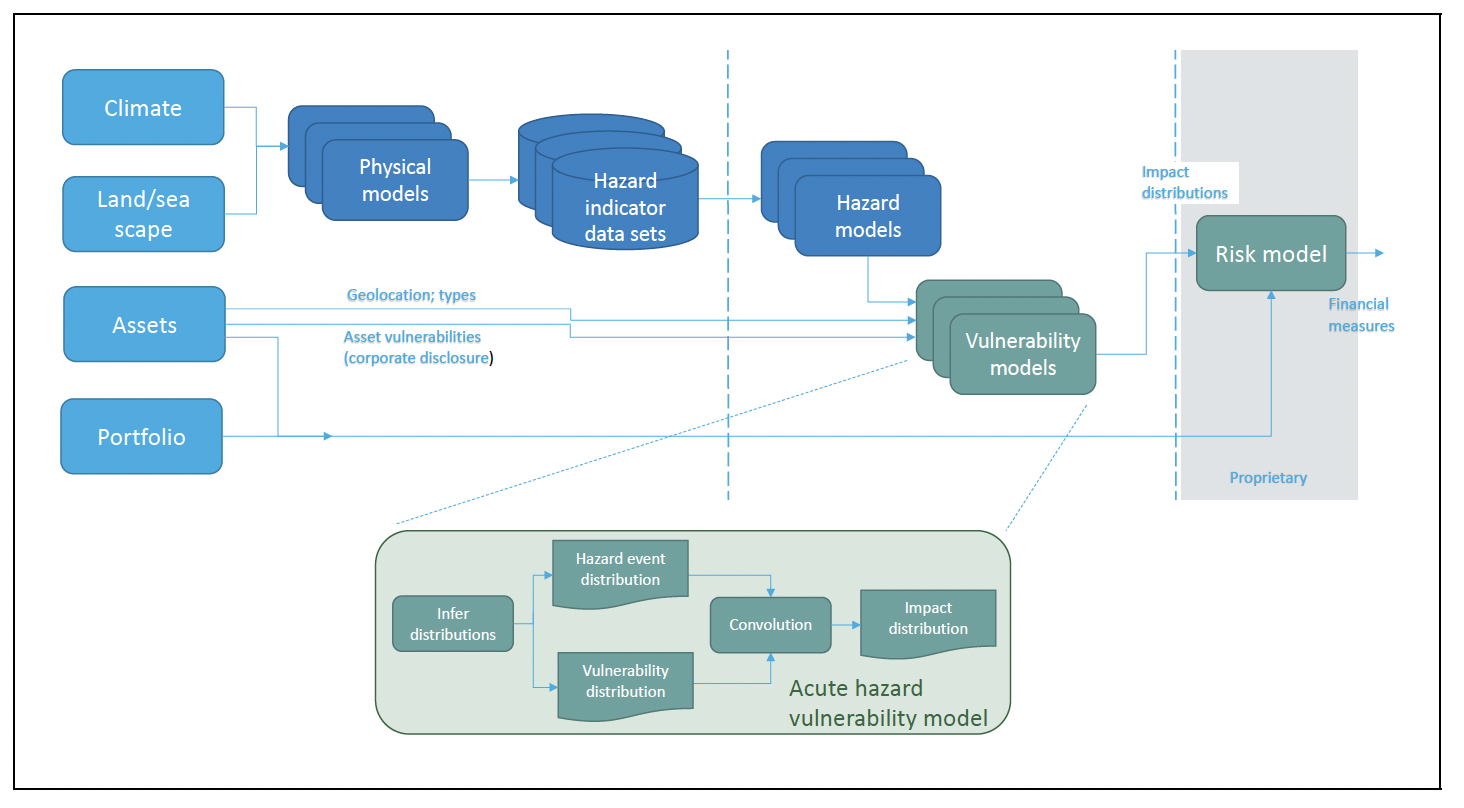
\includegraphics[width=0.9\textwidth]{figures/04/physrisk-overview-components.png}
    \caption[Physrisk physical risk model components.]{Conceptual architecture of a physical climate risk model, showing the integration of hazard data, vulnerability models, and asset-level exposure to produce impact distributions. Adapted from the CVAR Physrisk methodology \cite{moorhouse2024}.}
    \label{fig:physrisk-overview-components}
\end{figure}


\subsection{Data Flow and Model Interoperability}

Each flood model—whether global or local—is processed through the same onboarding interface, allowing standardization of outputs while preserving return-period-specific intensity information. The hazard models are structured into three-dimensional Zarr arrays indexed by latitude, longitude, and return period. This enables consistent querying and evaluation across models with different spatial resolutions or geographic coverage.

Once onboarded, all hazard layers become interchangeable within the Physrisk pipeline. Vulnerability models (e.g., depth--damage functions) and exposure datasets (e.g., building values or asset locations) can then be used in combination with any hazard source. This interoperability allows for both comparative experiments and compound risk evaluations, where multiple models are used to bound uncertainty or stress-test assumptions.

\subsection{Integration of the IKG Model}

The locally developed IKG model, originally provided in shapefile and GeoPackage vector formats, required a dedicated pre-processing stage to align with the Physrisk architecture. This process involved:
\begin{itemize}
    \item Transforming coordinate systems (from EPSG:3794 to EPSG:4326),
    \item Rasterizing vector layers into a fixed-resolution 5x5m grid,
    \item Assigning discrete flood depth values to each return period (RP10, RP100, RP500),
    \item Converting the raster layers into Zarr format for chunked cloud storage.
\end{itemize}

The unified model was then uploaded to AWS S3 and integrated into the Physrisk hazard module alongside WRI Aqueduct (and other, already onboarded models). This enabled direct comparison and batch evaluation of global versus local model predictions, described further in Section~\ref{sec:comparison-toolset}.

\begin{figure}[htb]
    \centering
    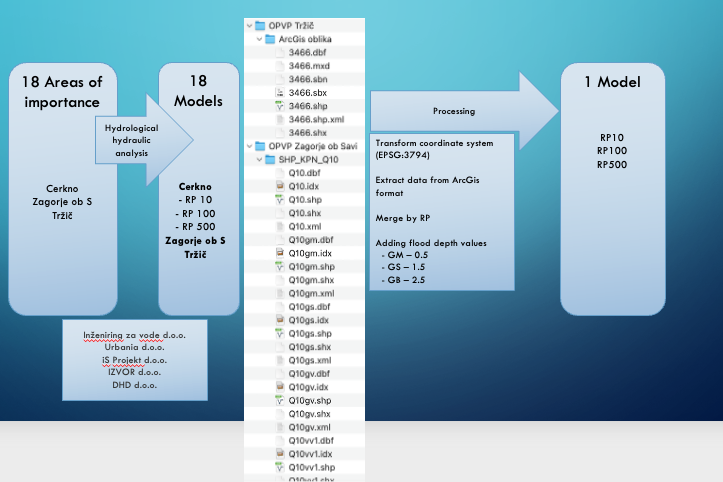
\includegraphics[width=0.95\textwidth]{figures/04/ikg_processing_pipeline.png}
    \caption[Processing heterogeneous IKG flood models.]{Pipeline for combining flood hazard data from 18 distinct Slovenian municipalities. Each area includes return-period-specific vector layers (e.g., shapefiles), which are transformed, reprojected, assigned standardized flood depth values (0.5 m, 1.5 m, 2.5 m), and merged into a single harmonized hazard model.}
    \label{fig:ikg_processing_pipeline}
\end{figure}

\subsection{Hazard Onboarding Pipeline}

The transformation from raw IKG data into a cloud-optimized flood hazard model is summarized in Figure~\ref{fig:ikg_physrisk_onboarding_pipeline}. The pipeline consists of the following steps:
\begin{enumerate}
    \item \textbf{Rasterization:} Converting input vector data into gridded raster tiles using a 5x5m resolution grid.
    \item \textbf{Zarrify:} Chunking the raster into 1000x1000 tiles and encoding into Zarr format.
    \item \textbf{Upload:} Transferring the data to AWS S3 for use within Physrisk.
\end{enumerate}

The final onboarded dataset can be queried via the Physrisk API or accessed directly for integration with ESG tools or batch model evaluation.

\begin{figure}[htb]
    \centering
    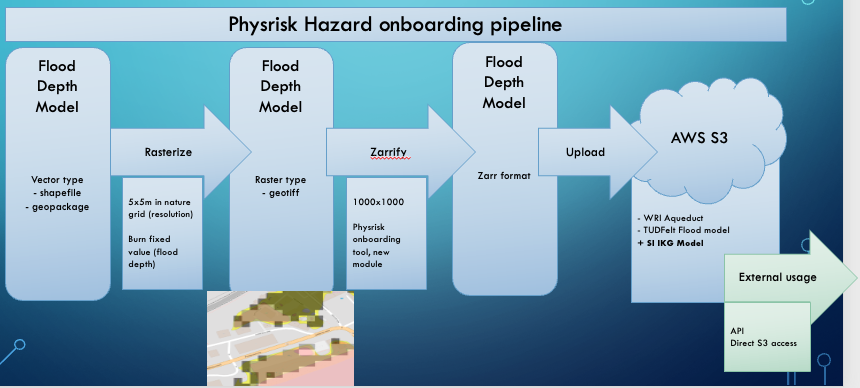
\includegraphics[width=0.9\textwidth]{figures/04/ikg_physrisk_onboarding_pipeline.png}
    \caption[Physrisk hazard onboarding pipeline.]{The onboarding pipeline for flood depth models into Physrisk. The process begins with vector data (e.g., shapefiles), rasterizes them into a 5x5 m resolution grid, converts to cloud-optimized Zarr format using the Physrisk onboarding tool, and uploads to AWS S3 for programmatic use.}
    \label{fig:ikg_physrisk_onboarding_pipeline}
\end{figure}

\section{Pipeline for Combining Heterogeneous IKG Models}

The \textit{Integralna karta globin} (IKG) flood hazard datasets are developed for individual municipalities or regions in Slovenia, each based on local hydrological and hydraulic analyses. These datasets differ in file structure, geospatial reference systems, data quality, and encoding of flood depths. To integrate these into a unified flood hazard model suitable for comparative evaluation and platform onboarding, a standardized processing pipeline was developed.

\subsection{Data Sources and Heterogeneity}

The raw IKG datasets were obtained from multiple engineering consultancies (\textit{Inženiring za vode d.o.o., Urbania d.o.o., iS Projekt d.o.o., IZVOR d.o.o., DHD d.o.o.}), each responsible for flood modeling in a subset of areas classified as "Območja pomembnega vpliva" (Areas of Significant Flood Risk) by Slovenian water authorities.

Each local model typically includes:
\begin{itemize}
    \item GIS vector data (shapefiles, GeoPackages) representing inundation zones,
    \item Attribute data encoding flood extent and classes for selected return periods (e.g., 10-, 100-, and 500-year events),
    \item Region-specific coordinate systems (typically EPSG:3794, Slovenia National Grid).
\end{itemize}

In total, data from 18 areas of importance were collected, with each area providing flood scenarios for three return periods. This resulted in 54 distinct layers that needed to be harmonized.

\subsection{Standardization and Processing Workflow}

To unify the IKG datasets into a single model, the following pipeline was developed and implemented in Python using open-source geospatial processing libraries (GDAL, Fiona, Rasterio, xarray):

\begin{enumerate}
    \item \textbf{Coordinate Transformation:} All source files were transformed from EPSG:3794 to WGS84 (EPSG:4326) to ensure compatibility with global models and standardized grid alignment.
    
    \item \textbf{Rasterization:} Vector layers were rasterized into a regular grid with a resolution of 5 meters (5x5m), which approximates the native resolution of the original hydrological models. A fixed flood depth value was assigned to each flood class:
    \begin{itemize}
        \item GM (minor flooding): 0.5 m
        \item GS (significant flooding): 1.5 m
        \item GB (severe flooding): 2.5 m
    \end{itemize}
    
    \item \textbf{Return Period Alignment:} Each rasterized layer was tagged with its associated return period (RP10, RP100, RP500). For each area, three separate rasters were produced and stacked by return period.
    
    \item \textbf{Tiling and Merging:} The processed rasters from all areas were mosaicked into a common spatial grid and stored as a 3D array indexed by latitude, longitude, and return period. Conflicts in overlapping regions (e.g., model boundaries) were resolved by assigning priority to higher-confidence datasets based on metadata quality.
\end{enumerate}

\subsection{Unified Flood Hazard Product}

The final result of this pipeline is a unified flood hazard model for Slovenia covering all 18 areas of importance for the 3 defined return periods. This model:
\begin{itemize}
    \item Captures flood depth estimates at high spatial resolution for three return periods,
    \item Standardizes input data from diverse local models into a single harmonized format,
    \item Enables consistent comparison with global models such as WRI Aqueduct within the same framework.
\end{itemize}

Figure~\ref{fig:ikg_processing_pipeline} provides a schematic representation of the transformation process, from raw shapefiles to a standardized hazard product.

This unified model was subsequently converted to Zarr format and onboarded into the Physrisk platform, as described in Section~\ref{sec:physrisk-framework-model-onboarding}.


%--------------------------------------------------------------------------------------------------
\section{Physrisk Framework – Model Onboarding}
\label{sec:physrisk-framework-model-onboarding}
%--------------------------------------------------------------------------------------------------

Once the local IKG flood models were unified into a standardized and spatially consistent format, the next step involved integrating them into the modular \textit{Physrisk} framework. Physrisk is part of the broader OS-Climate open-source ecosystem and is designed to facilitate scalable, scenario-based physical climate risk analysis. The framework separates hazard, vulnerability, and financial components and enables flexible model composition, comparison, and evaluation.

\subsection{Physrisk Architecture and Modules}

The Physrisk architecture is composed of several interoperable modules:

\begin{itemize}
    \item \textbf{OS-risk-hazard}: responsible for ingesting and formatting hazard data sets (e.g., flood depth by return period) into a common format.
    \item \textbf{OS-risk-physrisk}: computes impact distributions by convolving hazard data with vulnerability functions and exposure information.
    \item \textbf{OS-risk-financial}: translates physical impacts into financial metrics such as loss of asset value or disruption to operations.
    \item \textbf{Physrisk API}: exposes model outputs through a standardized programmatic interface.
\end{itemize}

The onboarding of hazard models occurs within the \texttt{os-risk-hazard} component and requires the hazard data to conform to a Zarr-based storage structure optimized for parallel access and spatial querying.

\subsection{Zarr Format and Indexing}

The Zarr format is a cloud-native format for storing large multi-dimensional arrays. It was chosen for hazard model storage due to its ability to:
\begin{itemize}
    \item Efficiently compress and store gridded data in chunks (e.g., 1000×1000 tiles),
    \item Allow selective download of spatial subsets,
    \item Support multi-indexing (e.g., latitude, longitude, return period).
\end{itemize}

For the unified IKG model, the hazard data were encoded into a 3-dimensional Zarr array with the following dimensions:
\begin{itemize}
    \item $i$: Latitude (y-axis),
    \item $j$: Longitude (x-axis),
    \item $k$: Return period index, corresponding to RP10, RP100, and RP500.
\end{itemize}

Each tile was stored as a compressed chunk and uploaded to an AWS S3-compatible bucket accessible to all Physrisk modules.

\subsection{Onboarding Procedure}

The onboarding process was implemented using the Physrisk hazard onboarding tool, a Python-based utility designed for structured hazard model integration. The steps were as follows:

\begin{enumerate}
    \item \textbf{Prepare Metadata:} Define the return periods, CRS (EPSG:4326), spatial resolution, and transformation matrix for the IKG model.
    
    \item \textbf{Convert to Zarr:} Use the onboarding tool to encode the processed GeoTIFF files into a Zarr store, assigning appropriate chunk sizes (e.g., 1000×1000 pixels).
    
    \item \textbf{Upload to Cloud Storage:} Transfer the Zarr directory to a cloud-accessible S3 bucket used by the OS-Climate infrastructure.
    
    \item \textbf{Register the Model:} Add a model reference entry into the hazard configuration of Physrisk, enabling downstream access via API and batch processors.
\end{enumerate}

\subsection{Integration with Other Models}

With the IKG model onboarded, it became available in the same infrastructure alongside global flood hazard layers, including:
\begin{itemize}
    \item WRI Aqueduct River Flood (global, ~1 km resolution),
    \item TU Delft River Flood (Pan-European, ~100 m resolution).
\end{itemize}

This interoperability allows any of the onboarded hazard layers to be used with common vulnerability functions and exposure datasets, enabling direct comparisons, uncertainty bounding, and ensemble evaluations. The IKG model is now fully accessible via the Physrisk API and can be used for property-level flood risk analysis in Slovenia under a unified modeling interface.

%--------------------------------------------------------------------------------------------------
\section{Comparison Toolset}
\label{sec:comparison-toolset}
%--------------------------------------------------------------------------------------------------

To evaluate and compare the predictive performance of flood hazard models, a model-agnostic comparison toolset was developed and integrated into the Physrisk framework. This toolset enables side-by-side querying of multiple hazard sources at specific geolocations and return periods, aligned with the reference flood observations used for validation in Chapter~5.

\subsection{Purpose and Design Principles}

The comparison toolset was designed with the following goals in mind:
\begin{itemize}
    \item \textbf{Model-agnostic access:} Allow querying of different onboarded hazard models (e.g., IKG, WRI Aqueduct) through a unified interface.
    \item \textbf{Return-period specificity:} Ensure comparability by extracting flood depth predictions at the same return period (e.g., 100-year flood).
    \item \textbf{Location-accurate evaluation:} Retrieve model outputs at high spatial precision to match reported flood locations.
    \item \textbf{Batch processing support:} Enable evaluation across hundreds of observations using efficient geospatial access patterns.
\end{itemize}

\subsection{Interface and Functionality}

The toolset consists of a lightweight Python interface built on top of the Physrisk hazard API. Given a set of coordinates (latitude, longitude) and a desired return period, the tool performs the following steps:

\begin{enumerate}
    \item \textbf{Coordinate Transformation:} Convert input coordinates into the grid index of the onboarded Zarr array using affine transformations defined in the model metadata.
    
    \item \textbf{Chunk Identification and Retrieval:} Locate the Zarr chunk containing the requested point and load the corresponding depth value for the specified return period.
    
    \item \textbf{Output Formatting:} Return the flood depth value, return period, and model metadata for downstream use in regression or classification analysis.
\end{enumerate}

When applied in batch mode, the tool leverages parallel reads and lazy loading to evaluate large datasets (e.g., the full validation set of flood reports) with minimal memory overhead.

\subsection{Supported Models and Inputs}

The toolset was validated for use with the following onboarded hazard models:

\begin{itemize}
    \item \textbf{SI IKG (Unified Model)}: High-resolution local flood model rasterized at 5x5 m, covering 18 Slovenian areas of importance, with RP10, RP100, and RP500 layers.
    \item \textbf{WRI Aqueduct Flood Hazard}: Global model with ~1 km resolution, scenario-aware, supporting multiple return periods from RP2 to RP1000.
\end{itemize}

The input to the toolset is a tabular dataset containing:
\begin{itemize}
    \item Latitude and longitude of each observation,
    \item Desired return period (e.g., RP100),
    \item Optional fields: timestamp, municipality, reported depth, reported damage.
\end{itemize}

\subsection{Integration with Validation Workflow}

The comparison outputs are stored in a structured table, allowing for direct computation of model performance metrics such as:
\begin{itemize}
    \item \textbf{Regression error:} difference between predicted and observed flood depths,
    \item \textbf{Classification accuracy:} match rate within flood depth categories (e.g., $<$0.5 m, 0.5–1.5 m, $>$1.5 m),
    \item \textbf{Bias analysis:} mean and median error segmented by proximity to water, terrain type, or municipality.
\end{itemize}

These outputs form the quantitative basis for the experimental results presented in Chapter~5.

\subsection{Reproducibility and Extensibility}

The toolset was developed as a standalone module and version-controlled as part of the project’s repository. This design ensures that future updates to hazard models (e.g., inclusion of climate scenario variants or additional regions) can be incorporated without changes to the validation logic.

Furthermore, the modularity of the toolset supports extension to:
\begin{itemize}
    \item Additional hazard types (e.g., pluvial flooding),
    \item Vulnerability assessments (via model chaining),
    \item Scenario-based risk projections (by switching hazard layers).
\end{itemize}

Thus, the comparison toolset serves not only as a core utility for this thesis, but also as a scalable evaluation framework for broader applications in physical climate risk modeling.

%
% Fifth chapter
\input{text-eng/main-chapter-5-ieee}
%
% Conclusions
%--------------------------------------------------------------------------------------------------
% 
\chapter{Conclusions \& Discussion}
%--------------------------------------------------------------------------------------------------

\section{Conclusion \& Interpretation of Results}

TBD


\section{Limitations of This Work}

TBD

\section{Future Work}

TBD
%--------------------------------------------------------------------------------------------------
%
% APPENDICES (optional)
%--------------------------------------------------------------------------------------------------
%
\appendix
\begin{appendices}
%
% For example, proofs of theorems could be an appendix
\input{text-eng/appendix-proofs}
%
\end{appendices}
%--------------------------------------------------------------------------------------------------
%
% BACK MATTER
%--------------------------------------------------------------------------------------------------
%
\backmatter
%
% References used in the thesis
\printreferences
% 
% Author's bibliography 
\input{text-eng/back-bibliography-ieee}
%
% Author's biography
\input{text-eng/back-biography}
%
% Index (optional)
\printmyindex
%--------------------------------------------------------------------------------------------------
\end{document}
%--------------------------------------------------------------------------------------------------
%
% MODIFICATION HISTORY
%--------------------------------------------------------------------------------------------------
% Version 1.3:
%  - Removed the sorting option from \printbibliography in IEEE bibliographies due to a new warning.
% Version 1.2: 
%  - Modified the symbols and abbreviations example to adjust the vertical positioning of the text
% Version 1.1: 
%  - Removed slovene.lbx and slovene-apa.lbx from accompanying files as they are now included in 
%    the latest biblatex version.
%  - Modified the bibliography example to include publications not referenced before.
%  - Modified the references example to show DOI should be used only for articles not yet published. 
%  - Modified the symbols and abbreviations example to accommodate long lines and long lists.
%  - Added pdf bookmarks for Acknowledgments, Abstract and Povzetek. 
%--------------------------------------------------------------------------------------------------
